%. . . . . . . . . . . . . . . . . . . . . . . . . . . . . . . . . . . . . . . . . . . . . . . . . . . . . . . . . . . . . . . . . . . . . . . . . . . . . . . . . . . . 
\section{Our Systematic mapping process}\label{sec:sm}
%. . . . . . . . . . . . . . . . . . . . . . . . . . . . . . . . . . . . . . . . . . . . . . . . . . . . . . . . . . . . . . . . . . . . . . . . . . . . . . . . . . . . 

%\iplacido{I changed the word expression `step' to `task' in order to describe
%the methodology `workflow'.}  
%We applied the systematic mapping methodology presented
% in~\cite{SM:Petersen:2008} to our study on SLA-guided data integration on a multi-cloud environments.

 
% \begin{description}
% \item \textbf{Definition of research question} to define the \textit{research scope};
% \item \textbf{Conduct search} in order to retrieve \textit{all candidate papers}. Those papers are selected applying a query which express the research interest to scientific databases;
% \item  \textbf{Screening of papers} to select the \textit{relevant papers} to answer the research question based on a inclusion and exclusion criteria;
% \item \textbf{Keywording using abstracts} to identify terms that helps on developing the \textit{classification scheme} (mapping categories to classify the papers); and
% \item \textbf{Data extraction and mapping process} to sort the relevant papers into the mapping categories and produce the systematic mapping.
% \end{description}

% The following subsections describes our first to fourth step in the
% mapping. %The systematic mapping results are presented in the next section.   



%As mentioned before, the aim of our systematic mapping process is first to
%check how \textit{SLA-guided data integration on a
%multi-cloud environments} has been explored in the literature, and discover
%possible gaps and issues.

The aim of our bibliographic study using the systematic mapping methodology \cite{SM:Petersen:2008}  is to identify   the key contributions and the evolution of the research done on \textit{SLA-guided
data integration on a multi-cloud environments} and discover open issues and limitations of existing work.    
Our study is guided by  three research questions:
%In order to achieve this goal we formulated three research questions:

\paragraph{\textit{\textbf{RQ1:} Which are the SLA measures that have been mostly
applied  in the cloud?}} This question will help  to identify  the type of properties used for characterizing and evaluating the services provided  by different clouds and the type of measures used for evaluating these properties and expressed in service level agreements.


\paragraph{ \textit{\textbf{RQ2:}  How have published papers on data
 integration evolved towards cloud topics?}} This question is devoted to identify the way  data integration problems addressed in the literature started  to include issues introduced by the cloud.

\paragraph{\textit{\textbf{RQ3:} In which way and in which context has data integration been linked to Quality of Service (QoS) measures in the literature?}} The objective of this question is to understand which QoS measures have been used for evaluating data integration and to determine the conditions in which  specific measures are particularly used.

%--------------------------------------------------------------------------------------------------------------------------------------------
\subsection{Search and screening of papers} \label{subsec:search}
%--------------------------------------------------------------------------------------------------------------------------------------------

According to our research questions and our expertise in data integration we chose a set of keywords to define a complex query to be used for retrieving papers from four target publications databases: IEEE~\footnote{http://ieeexplore.ieee.org/},
ACM~\footnote{http://dl.acm.org/}, Science Direct~\footnote{http://www.sciencedirect.com/} and
CiteSeerX~\footnote{http://citeseerx.ist.psu.edu/}. We used the following conjunctive and disjunctive general query which was completed with associated terms from a thesaurus and rewritten according to the expression rules of advanced queries in each database: 


%\medskip
%\begin{small}
%\begin{verbatim}
%(("SLA" OR "Service Level Agreement" OR "Service-Level Agreement") AND 
%   ("Cloud" OR "Multi-cloud" OR "Multi cloud" OR "Multicloud" OR "Inter-cloud" OR 
%      "Inter cloud" OR "Intercloud" OR "Federated cloud" OR "Cloud federation" OR 
%         "Hybrid cloud")) OR
%(("SLA" OR "Service Level Agreement" OR "Service-Level Agreement") AND 
%   ("Data Integration" OR "Data Integration Systems" OR "Sources Integration" OR 
%      "Multi Databases" OR "Multi-databases" OR "Multidatabases" OR 
%         "Distributed databases")) OR
%(("Data Integration" OR "Data Integration Systems" OR "Sources Integration" OR 
%   "Multi Databases" OR "Multi-databases" OR "Multidatabases" OR 
%      "Distributed databases") AND 
%   ("Cloud" OR "Multi-cloud" OR "Multi cloud" OR "Multicloud" OR "Inter-cloud" OR 
%      "Inter cloud" OR "Intercloud" OR "Federated cloud" OR "Cloud federation" OR 
%        "Hybrid cloud")) OR
%(("Data Integration" OR "Data Integration Systems" OR "Sources Integration" OR 
%   "Multi Databases" OR "Multi-databases" OR "Multidatabases" OR 
%      "Distributed databases") AND 
%   ("QoS" and "Quality of Service"))
%\end{verbatim}
%\end{small}
%\daniel{New format of the query. We saved some space.}

%\begin{small}
%\textit{(("SLA" OR "Service Level Agreement" OR "Service-Level Agreement") AND 
%   ("Cloud" OR "Multi-cloud" OR "Multi cloud" OR "Multicloud" OR "Inter-cloud" OR 
%      "Inter cloud" OR "Intercloud" OR "Federated cloud" OR "Cloud federation" OR 
%\medskip        "Hybrid cloud"))} \textbf{OR} \\ 
%\textit{(("SLA" OR "Service Level Agreement" OR "Service-Level Agreement") AND 
%   ("Data Integration" OR "Data Integration Systems" OR "Sources Integration" OR 
%      "Multi Databases" OR "Multi-databases" OR "Multidatabases" OR }
%\medskip        \textit{ "Distributed databases"))} \textbf{OR} \\
%\textit{(("Data Integration" OR "Data Integration Systems" OR "Sources Integration" OR 
%   "Multi Databases" OR "Multi-databases" OR "Multidatabases" OR 
%      "Distributed databases") AND 
%   ("Cloud" OR "Multi-cloud" OR "Multi cloud" OR "Multicloud" OR "Inter-cloud" OR 
%      "Inter cloud" OR "Intercloud" OR "Federated cloud" OR "Cloud federation" OR }
%\medskip       \textit{ "Hybrid cloud"))} \textbf{OR} \\
%\textit{(("Data Integration" OR "Data Integration Systems" OR "Sources Integration" OR 
%   "Multi Databases" OR "Multi-databases" OR "Multidatabases" OR 
%      "Distributed databases") AND 
%   ("QoS" and "Quality of Service"))}
%\end{small}
%\medskip

\begin{center}
\textit{("Service level agreement"  AND "Data integration" AND "Database integration" AND "Cloud" AND "Multi-cloud ")} \\ 
\end{center}
\medskip

%Considering that each scientific database has different search engines, the general query was 
%rewritten in several manners according to each database syntax.
%We searched and filtered relevant works in four steps.
%In the first step we searched in four scientific databases: IEEE~\footnote{http://ieeexplore.ieee.org/},
%ACM~\footnote{http://dl.acm.org/}, Science Direct~\footnote{http://www.sciencedirect.com/} and
%We retrieved 1832 publications (See table~\ref{table:pub}).


\begin{table}[!ht]
\begin{center}
\begin{tabular}{>{\centering\arraybackslash}p{2.5cm}|>{\centering\arraybackslash}p{2.5cm}|>{\centering\arraybackslash}p{2.5cm}|>{\centering\arraybackslash}p{2.5cm}}
\toprule
\textbf{Database} & \textbf{Amount} & \textbf{Included} & \textbf{Excluded} \\ 
\hline \toprule
\textbf{IEEE} & 658 & 56 & 602 \\ 
\hline 
\textbf{AMC} & 649 & 31 & 618	 \\ 
\hline 
\textbf{Science Direct} & 106 & 6 & 100 \\ 
\hline 
\textbf{CiteSeerX} & 419 & 21 & 398 \\ 
\hline 
\textit{Total} & 1832 & \textbf{114} & 1718 \\ 
\bottomrule \hline
\end{tabular} 
\end{center}
\caption{Number of papers retrieved in each scientific database}\label{table:pub}
\end{table}

We retrieved  a total of 1832 publications shown in Table~\ref{table:pub}. According to the systematic mapping methodology, the initial collection was cleaned and filtered according to inclusion and exclusion criteria applied as filters when analyzing the titles and abstracts of the papers. 
%(see table~\ref{table:criteria}).  
In general, we only kept publications written in English, addressing SLA models and languages, quality measures, and/or (multi)-cloud topics related to data integration. As a result of the filtering process we excluded 1718 publications. 
The columns \textit{Included} and \textit{Excluded} in Table~\ref{table:pub} summarize the number of papers per database that were included and excluded for building the final collection with  114 publications.


%\begin{table}[!htb]
%\begin{center}
%\begin{tabular}{p{10cm}}
%\bottomrule \hline
%\textbf{Inclusion criteria} \\ 
%\hline 
%- The text must be in English \\ 
%- SLA approaches including data integration and/or multi-cloud environments\\
%- Studies regarding SLA and cloud, describing models, languages and security issues \\
%- Works describing improvements to SLA \\
%- Data integration studies including cloud and/or multi-cloud  \\
%- Quality of Service efforts regarding data integration \\
%\bottomrule \hline 
%\textbf{Exclusion criteria} \\ 
%\hline 
%- Publication with only power point version available \\ 
%- SLA approaches regarding resource allocation \\
%- Any paper out of the inclusion criteria  \\
%\bottomrule \hline
%\end{tabular} 
%\end{center}
%\caption{Inclusion and exclusion criteria}\label{table:criteria}
%\end{table}

%--------------------------------------------------------------------------------------------------------------------------------------------
\subsection{Defining a classification scheme}
%--------------------------------------------------------------------------------------------------------------------------------------------

We analyzed the titles and abstracts of the papers of the corpus que derived in the previous phase using information retrieval techniques in order to identify the frequent relevant terms. We used this terms for building a classification scheme consisting of five facets that group frequent relevant terms. According to the systematic mapping methodology, the relevant frequent terms can be considered as dimensions that represent subcategories within the facets that group them. We define the facets and dimensions of the classification scheme that we propose for studying SLA guided data integration in multi-cloud environments.
%According to our research interests, these papers were classified using the five facets. 
%The facets' dimensions were defined based on our knowledge and on the keywording process proposed by the
%methodology.  
%Each facet has its own dimensions. 
%These dimensions were proposed based on our knowledge and on the keywords found in the abstracts.   

%.  -   .  .  -   ..  -   ..  -   ..  -   ..  -   ..  -   ..  -   ..  -   ..  -   ..  -   ..  -   ..  -   ..  -   ..  -   ..  -   ..  -   ..  -   ..  -   ..  -   ..  -   ..  -   ..  -   ..  -   .  
\paragraph{Data Integration Environment}  
%.  -   .  .  -   ..  -   ..  -   ..  -   ..  -   ..  -   ..  -   ..  -   ..  -   ..  -   ..  -   ..  -   ..  -   ..  -   ..  -   ..  -   ..  -   ..  -   ..  -   ..  -   ..  -   ..  -   ..  -   .  
%As shown in table~\ref{table:dienviron} 
This facet groups the dimensions that characterize the architectures used for delivering data integration services ({\em data warehouse} and  {\em federated database}) and  architectures used for deploying these services ({\em cloud} and {\em multi-cloud}).
%\begin{table}[h]
%\begin{center}
%\begin{tabular}{p{4cm}p{10cm}}
%\hline 
%\textbf{Dimension} & \textbf{Publication} \\ 
%\hline 
%Cloud & 
%\cite{106,110,105,107,108,109,068,070,072,113,073,074,075,076,077,078,079,081,082,083,085,087,088,089,090,094,095,096,097,098,099,100,102,103}\\ 
%\hline 
%Data Warehouse & \cite{066,114,091} \\ 
%\hline 
%Federated Database & \cite{071,089,112} \\ 
%\hline 
%Multi-cloud & \cite{012,071,093} \\ 
%\hline 
%\end{tabular}
%\end{center}
%\caption{Data Integration Environment facet}\label{table:dienviron}
%\end{table}

%\begin{table}[!h]
%\begin{center}
%\begin{tabular}{p{4cm}p{4cm}}
%\hline 
%\textbf{Dimension} & \textbf{Publication} \\ 
%\hline 
%Cloud & 34 \\ 
%\hline 
%Data Warehouse & 3 \\ 
%\hline 
%Federated Database & 3 \\ 
%\hline 
%Multi-cloud & 3 \\ 
%\hline 
%\end{tabular}
%\end{center}
%\caption{Data Integration Environment facet:  papers per dimension}\label{table:dienviron}
%\end{table}

%.  -   .  .  -   ..  -   ..  -   ..  -   ..  -   ..  -   ..  -   ..  -   ..  -   ..  -   ..  -   ..  -   ..  -   ..  -   ..  -   ..  -   ..  -   ..  -   ..  -   ..  -   ..  -   ..  -   ..  -   .  
\paragraph{Data Integration Description}
%.  -   .  .  -   ..  -   ..  -   ..  -   ..  -   ..  -   ..  -   ..  -   ..  -   ..  -   ..  -   ..  -   ..  -   ..  -   ..  -   ..  -   ..  -   ..  -   ..  -   ..  -   ..  -   ..  -   ..  -   .  
 %As shown in table~\ref{table:didesc} 
 This facet groups the dimensions describing the type of data used for describing the databases content in order to  integrate them. Data integration can be done by using {\em meta-data, schema}, and {\em knowledge}.
%\begin{table}[h]
%\begin{center}
%\begin{tabular}{p{4cm}p{10cm}}
%\hline 
%\textbf{Dimension} & \textbf{Publication} \\ 
%\hline 
%Knowledge & \cite{012,083} \\ 
%\hline 
%Metadata & \cite{108,066,113} \\ 
%\hline 
%Schema & \cite{070,071,072,073,075,114,083,089,091,112,102} \\ 
%\hline 
%\end{tabular}
%\end{center}
%\caption{Data Integration Description facet}\label{table:didesc}
%\end{table}

%\begin{table}[!h]
%\begin{center}
%\begin{tabular}{p{4cm}p{4cm}}
%\hline 
%\textbf{Dimension} & \textbf{Publication} \\ 
%\hline 
%Knowledge & 2 \\ 
%\hline 
%Metadata & 3 \\ 
%\hline 
%Schema & 11 \\ 
%\hline 
%\end{tabular}
%\end{center}
%\caption{Data Integration Description facet: papers per dimension}\label{table:didesc}
%\end{table}

%.  -   .  .  -   ..  -   ..  -   ..  -   ..  -   ..  -   ..  -   ..  -   ..  -   ..  -   ..  -   ..  -   ..  -   ..  -   ..  -   ..  -   ..  -   ..  -   ..  -   ..  -   ..  -   ..  -   ..  -   .  
\paragraph{Data Quality} 
%.  -   .  .  -   ..  -   ..  -   ..  -   ..  -   ..  -   ..  -   ..  -   ..  -   ..  -   ..  -   ..  -   ..  -   ..  -   ..  -   ..  -   ..  -   ..  -   ..  -   ..  -   ..  -   ..  -   ..  -   .  
%As shown in table~\ref{table:dq} 
This facet groups the dimensions that represent the parameters that can be used for measuring data quality. Measures can be related directly to data for instance {\em confidentiality, privacy, security, protection and provenance} and to the conditions in which data is integrated and delivered  (i.e., dimension {\em SLA}).
%Note that a publication is classified in the SLA dimension when it does not focus on a specific quality parameter, but in general uses a SLA contract in order to specify one or more.
%\begin{table}[h]
%\begin{center}
%\begin{tabular}{p{4cm}p{10cm}}
%\hline 
%\textbf{Dimension} & \textbf{Publication} \\ 
%\hline 
%Confidentiality & \cite{104,109,111,024} \\ 
%\hline 
%Privacy & \cite{109,111,007,067,068,113,024,047,095,096} \\ 
%\hline 
%Security & \cite{109,113,081,093,112,065} \\ 
%\hline 
%SLA  &\cite{044,001,002,007,008,009,011,012,013,014,015,016,017,018,019,046,020,021,022,024,025,026,027,028,029,030,031,032,035,034,036,037,038,039,040,041,042,023,043,045,047,048,049,050,051,052,053,054,055,056,057,058,060,059,061,062,063,064,065,033}\\
%\hline 
%Data Protection & \cite{106,104,047} \\ 
%\hline 
%Data Provenance & \cite{012} \\ 
%\hline 
%Others & \cite{071,093,100} \\ 
%\hline 
%\end{tabular}
%\end{center}
%\caption{Data Quality facet}\label{table:dq}
%\end{table}

%\begin{table}[!h]
%\begin{center}
%\begin{tabular}{p{4cm}p{4cm}}
%\hline 
%\textbf{Dimension} & \textbf{Publication} \\ 
%\hline 
%Confidentiality & 4 \\ 
%\hline 
%Privacy & 10 \\ 
%\hline 
%Security & 6 \\ 
%\hline 
%SLA  & 60\\
%\hline 
%Data Protection & 3 \\ 
%\hline 
%Data Provenance & 1 \\ 
%\hline 
%Others & 3 \\ 
%\hline 
%\end{tabular}
%\end{center}
%\caption{Data Quality: papers per dimension}\label{table:dq}
%\end{table}

%.  -   .  .  -   ..  -   ..  -   ..  -   ..  -   ..  -   ..  -   ..  -   ..  -   ..  -   ..  -   ..  -   ..  -   ..  -   ..  -   ..  -   ..  -   ..  -   ..  -   ..  -   ..  -   ..  -   ..  -   .  
\paragraph{SLA expression}
%.  -   .  .  -   ..  -   ..  -   ..  -   ..  -   ..  -   ..  -   ..  -   ..  -   ..  -   ..  -   ..  -   ..  -   ..  -   ..  -   ..  -   ..  -   ..  -   ..  -   ..  -   ..  -   ..  -   ..  -   .  
  refers to the contracted delivery time of the service or its performance. It represents agreements between the user and a system expressed as a combination of weighted measures. 
%As shown in Table~\ref{table:sla} 
This facet groups dimensions describing the way SLA is represented in order to associate it to service provision.
SLA can be expressed using a  {\em language},  {\em model}, {\em resources} concerned by SLA and degree of  {\em security} provided by a data integration service.

%\begin{table}[h]
%\begin{center}
%\begin{tabular}{p{4cm}p{10cm}}
%\hline 
%\textbf{Dimension} & \textbf{Publication} \\ 
%\hline 
%Language & \cite{003,037,039,041,055,056,061} \\ 
%\hline 
%Model & \cite{044,001,002,005,003,006,007,008,009,010,012,013,014,015,016,017,018,019,046,020,021,022,024,026,027,028,029,030,031,032,035,036,038,040,042,023,043,045,047,048,049,050,051,053,054,055,057,058,060,059,061,063,033}\\ 
%\hline 
%Resources & \cite{110,053,064} \\ 
%\hline 
%Security & \cite{109,011,113,025,035,034,081,038,049,050,052,093,062,112,065} \\ 
%\hline 
%\end{tabular}
%\end{center}
%\caption{SLA facet}\label{table:sla}
%\end{table}

%\begin{table}[h]
%\begin{center}
%\begin{tabular}{p{4cm}p{4cm}}
%\hline 
%\textbf{Dimension} & \textbf{Publication} \\ 
%\hline 
%Language & 7 \\ 
%\hline 
%Model & 53 \\ 
%\hline 
%Resources & 3 \\ 
%\hline 
%Security & 15 \\ 
%\hline 
%\end{tabular}
%\end{center}
%\caption{SLA expression facet: papers per dimension}\label{table:sla}
%\end{table}

%.  -   .  .  -   ..  -   ..  -   ..  -   ..  -   ..  -   ..  -   ..  -   ..  -   ..  -   ..  -   ..  -   ..  -   ..  -   ..  -   ..  -   ..  -   ..  -   ..  -   ..  -   ..  -   ..  -   ..  -   .  
\paragraph{Contribution} 
%.  -   .  .  -   ..  -   ..  -   ..  -   ..  -   ..  -   ..  -   ..  -   ..  -   ..  -   ..  -   ..  -   ..  -   ..  -   ..  -   ..  -   ..  -   ..  -   ..  -   ..  -   ..  -   ..  -   ..  -   .  
%As shown in table~\ref{table:contribution} 
This facet groups dimensions representing the kind of contribution proposed for addressing data integration. Contributions can concern abstractions like a
  {\em method}, a  {\em model}, or a {\em process}, software {\em tools} or bibliographic and systems analysis like {\em literature analysis} and {\em extended studies}.
%\begin{table}[h]
%\begin{center}
%\begin{tabular}{p{4cm}p{10cm}}
%\hline 
%\textbf{Dimension} & \textbf{Publication} \\ 
%\hline 
%Tool & \cite{110,001,002,005,066,068,070,071,011,014,015,016,019,046,113,024,074,077,026,078,028,029,032,035,081,086,087,088,053,054,091,056,093,094,095,061,112,064,065}\\ 
%\hline 
%Literature Analysis & \cite{105,108,109,111,004,003,069,010,073,038,042,089,048,052,099,103} \\ 
%\hline 
%Method & \cite{106,107,011,075,076,043,051,092,101,102} \\ 
%\hline 
%Model & \cite{044,006,007,066,067,008,009,070,012,071,072,013,017,018,020,114,027,079,030,031,034,036,080,082,037,083,084,039,040,085,041,087,088,045,090,049,050,055,056,057,058,060,059,096,062,098,063,033}\\  
%\hline 
%Process & \cite{021,022,025,023,096,100} \\ 
%\hline 
%Extended Study & \cite{104,047,097} \\ 
%\hline 
%\end{tabular}
%\end{center}
%\caption{Contribution facet}\label{table:contribution}
%\end{table}

%\begin{table}[h]
%\begin{center}
%\begin{tabular}{p{4cm}p{4cm}}
%\hline 
%\textbf{Dimension} & \textbf{Publication} \\ 
%\hline 
%Tool & 39\\ 
%\hline 
%Literature Analysis & 16 \\ 
%\hline 
%Method & 10 \\ 
%\hline 
%Model & 48 \\  
%\hline 
%Process & 6 \\ 
%\hline 
%Extended Study & 3 \\ 
%\hline 
%\end{tabular}
%\end{center}
%\caption{Contribution facet: papers per dimension}\label{table:contribution}
%\end{table}

%.  -   .  .  -   ..  -   ..  -   ..  -   ..  -   ..  -   ..  -   ..  -   ..  -   ..  -   ..  -   ..  -   ..  -   ..  -   ..  -   ..  -   ..  -   ..  -   ..  -   ..  -   ..  -   ..  -   ..  -   .  
\paragraph{Paper type}
%.  -   .  .  -   ..  -   ..  -   ..  -   ..  -   ..  -   ..  -   ..  -   ..  -   ..  -   ..  -   ..  -   ..  -   ..  -   ..  -   ..  -   ..  -   ..  -   ..  -   ..  -   ..  -   ..  -   ..  -   .  
%As shown in   Table~\ref{table:research} 
This facet groups dimensions representing the type and purpose of the papers that address data integration: {\em evaluation, validation, solution} and {\em  position}.

%\begin{table}[h]
%\begin{center}
%\begin{tabular}{p{4cm}p{10cm}}
%\hline 
%\textbf{Dimension} & \textbf{Publication} \\ 
%\hline 
%Evaluation research & \cite{008,026,048,069,073,074,089,094,099,102,103,105,111} \\ 
%\hline 
%Validation research & \cite{001,002,005,006,007,009,011,012,014,015,016,017,018,019,020,021,022,023,024,025,027,028,029,030,031,032,033,034,036,037,039,045,051,057,059,079,095,098,100,105,112}\\
%\hline 
%Solution proposal & \cite{008,035,038,040,041,042,043,044,046,047,048,049,050,051,053,054,055,056,058,060,061,062,063,064,065,066,067,068,070,071,072,075,076,077,078,079,080,081,082,083,084,085,086,087,088,090,091,092,093,094,095,096,097,098,100,101,102,104,106,107,110,113,114}\\
%\hline 
%Opinion paper & \cite{003,004,010,013,052,069,073,108,109} \\ 
%\hline  
%\end{tabular}
%\end{center}
%\caption{Research facet}\label{table:research}
%\end{table}

%\begin{table}[h]
%\begin{center}
%\begin{tabular}{p{4cm}p{4cm}}
%\hline 
%\textbf{Dimension} & \textbf{Publication} \\ 
%\hline 
%Evaluation research & 13 \\ 
%\hline 
%Validation research & 41 \\
%\hline 
%Solution proposal & 63\\
%\hline 
%Opinion paper & 9 \\ 
%\hline  
%\end{tabular}
%\end{center}
%\caption{Paper type facet: papers per dimension}\label{table:research}
%\end{table}

%\idaniel{New table...}
%\begin{table}[!h]
%\begin{center}
%\begin{tabular}{p{4cm}p{10cm}}
%\hline 
%\textbf{Dimension} & \textbf{Publication} \\ 
%\hline 
%Cloud & 
%\cite{106,110,105,107,108,109,068,070,072,113,073,074,075,076,077,078,079,081,082,083,085,087,088,089,090,094,095,096,097,098,099,100,102,103}\\ 
%\hline 
%Data Warehouse & \cite{066,114,091} \\ 
%\hline 
%Federated Database & \cite{071,089,112} \\ 
%\hline 
%Multi-cloud & \cite{012,071,093} \\ 
%\hline 
%\hline 
%Knowledge & \cite{012,083} \\ 
%\hline 
%Metadata & \cite{108,066,113} \\ 
%\hline 
%Schema & \cite{070,071,072,073,075,114,083,089,091,112,102} \\ 
%\hline 
%\hline 
%Confidentiality & \cite{104,109,111,024} \\ 
%\hline 
%Privacy & \cite{109,111,007,067,068,113,024,047,095,096} \\ 
%\hline 
%Security & \cite{109,113,081,093,112,065} \\ 
%\hline 
%SLA  &\cite{044,001,002,007,008,009,011,012,013,014,015,016,017,018,019,046,020,021,022,024,025,026,027,028,029,030,031,032,035,034,036,037,038,039,040,041,042,023,043,045,047,048,049,050,051,052,053,054,055,056,057,058,060,059,061,062,063,064,065,033}\\
%\hline 
%Data Protection & \cite{106,104,047} \\ 
%\hline  
%Data Provenance & \cite{012} \\ 
%\hline 
%Others & \cite{071,093,100} \\ 
%\hline 
%\hline 
%Language & \cite{003,037,039,041,055,056,061} \\ 
%\hline 
%Model & \cite{044,001,002,005,003,006,007,008,009,010,012,013,014,015,016,017,018,019,046,020,021,022,024,026,027,028,029,030,031,032,035,036,038,040,042,023,043,045,047,048,049,050,051,053,054,055,057,058,060,059,061,063,033}\\ 
%\hline 
%Resources & \cite{110,053,064} \\ 
%\hline 
%Security & \cite{109,011,113,025,035,034,081,038,049,050,052,093,062,112,065} \\ 
%\hline
%\hline 
%Tool & \cite{110,001,002,005,066,068,070,071,011,014,015,016,019,046,113,024,074,077,026,078,028,029,032,035,081,086,087,088,053,054,091,056,093,094,095,061,112,064,065}\\ 
%\hline 
%Literature Analysis & \cite{105,108,109,111,004,003,069,010,073,038,042,089,048,052,099,103} \\ 
%\hline 
%Method & \cite{106,107,011,075,076,043,051,092,101,102} \\ 
%\hline 
%Model & \cite{044,006,007,066,067,008,009,070,012,071,072,013,017,018,020,114,027,079,030,031,034,036,080,082,037,083,084,039,040,085,041,087,088,045,090,049,050,055,056,057,058,060,059,096,062,098,063,033}\\  
%\hline 
%Process & \cite{021,022,025,023,096,100} \\ 
%\hline 
%Extended Study & \cite{104,047,097} \\ 
%\hline 
%\hline 
%Evaluation research & \cite{008,026,048,069,073,074,089,094,099,102,103,105,111} \\ 
%\hline 
%Validation research & \cite{001,002,005,006,007,009,011,012,014,015,016,017,018,019,020,021,022,023,024,025,027,028,029,030,031,032,033,034,036,037,039,045,051,057,059,079,095,098,100,105,112}\\
%\hline 
%Solution proposal & \cite{008,035,038,040,041,042,043,044,046,047,048,049,050,051,053,054,055,056,058,060,061,062,063,064,065,066,067,068,070,071,072,075,076,077,078,079,080,081,082,083,084,085,086,087,088,090,091,092,093,094,095,096,097,098,100,101,102,104,106,107,110,113,114}\\
%\hline 
%Opinion paper & \cite{003,004,010,013,052,069,073,108,109} \\ 
%\hline  
%\end{tabular}
%\end{center}
%\caption{List of publications per dimension}\label{table:dimensions}

%\end{table}

Facets define the classification scheme we used for  classifying the papers in the corpus according to dimensions. 
Each paper can be classified into one or several dimensions of each facet. 
%Tables \ref{table:dienviron} to \ref{table:research} summarize the classification results.

\begin{figure}[h!]
\centering
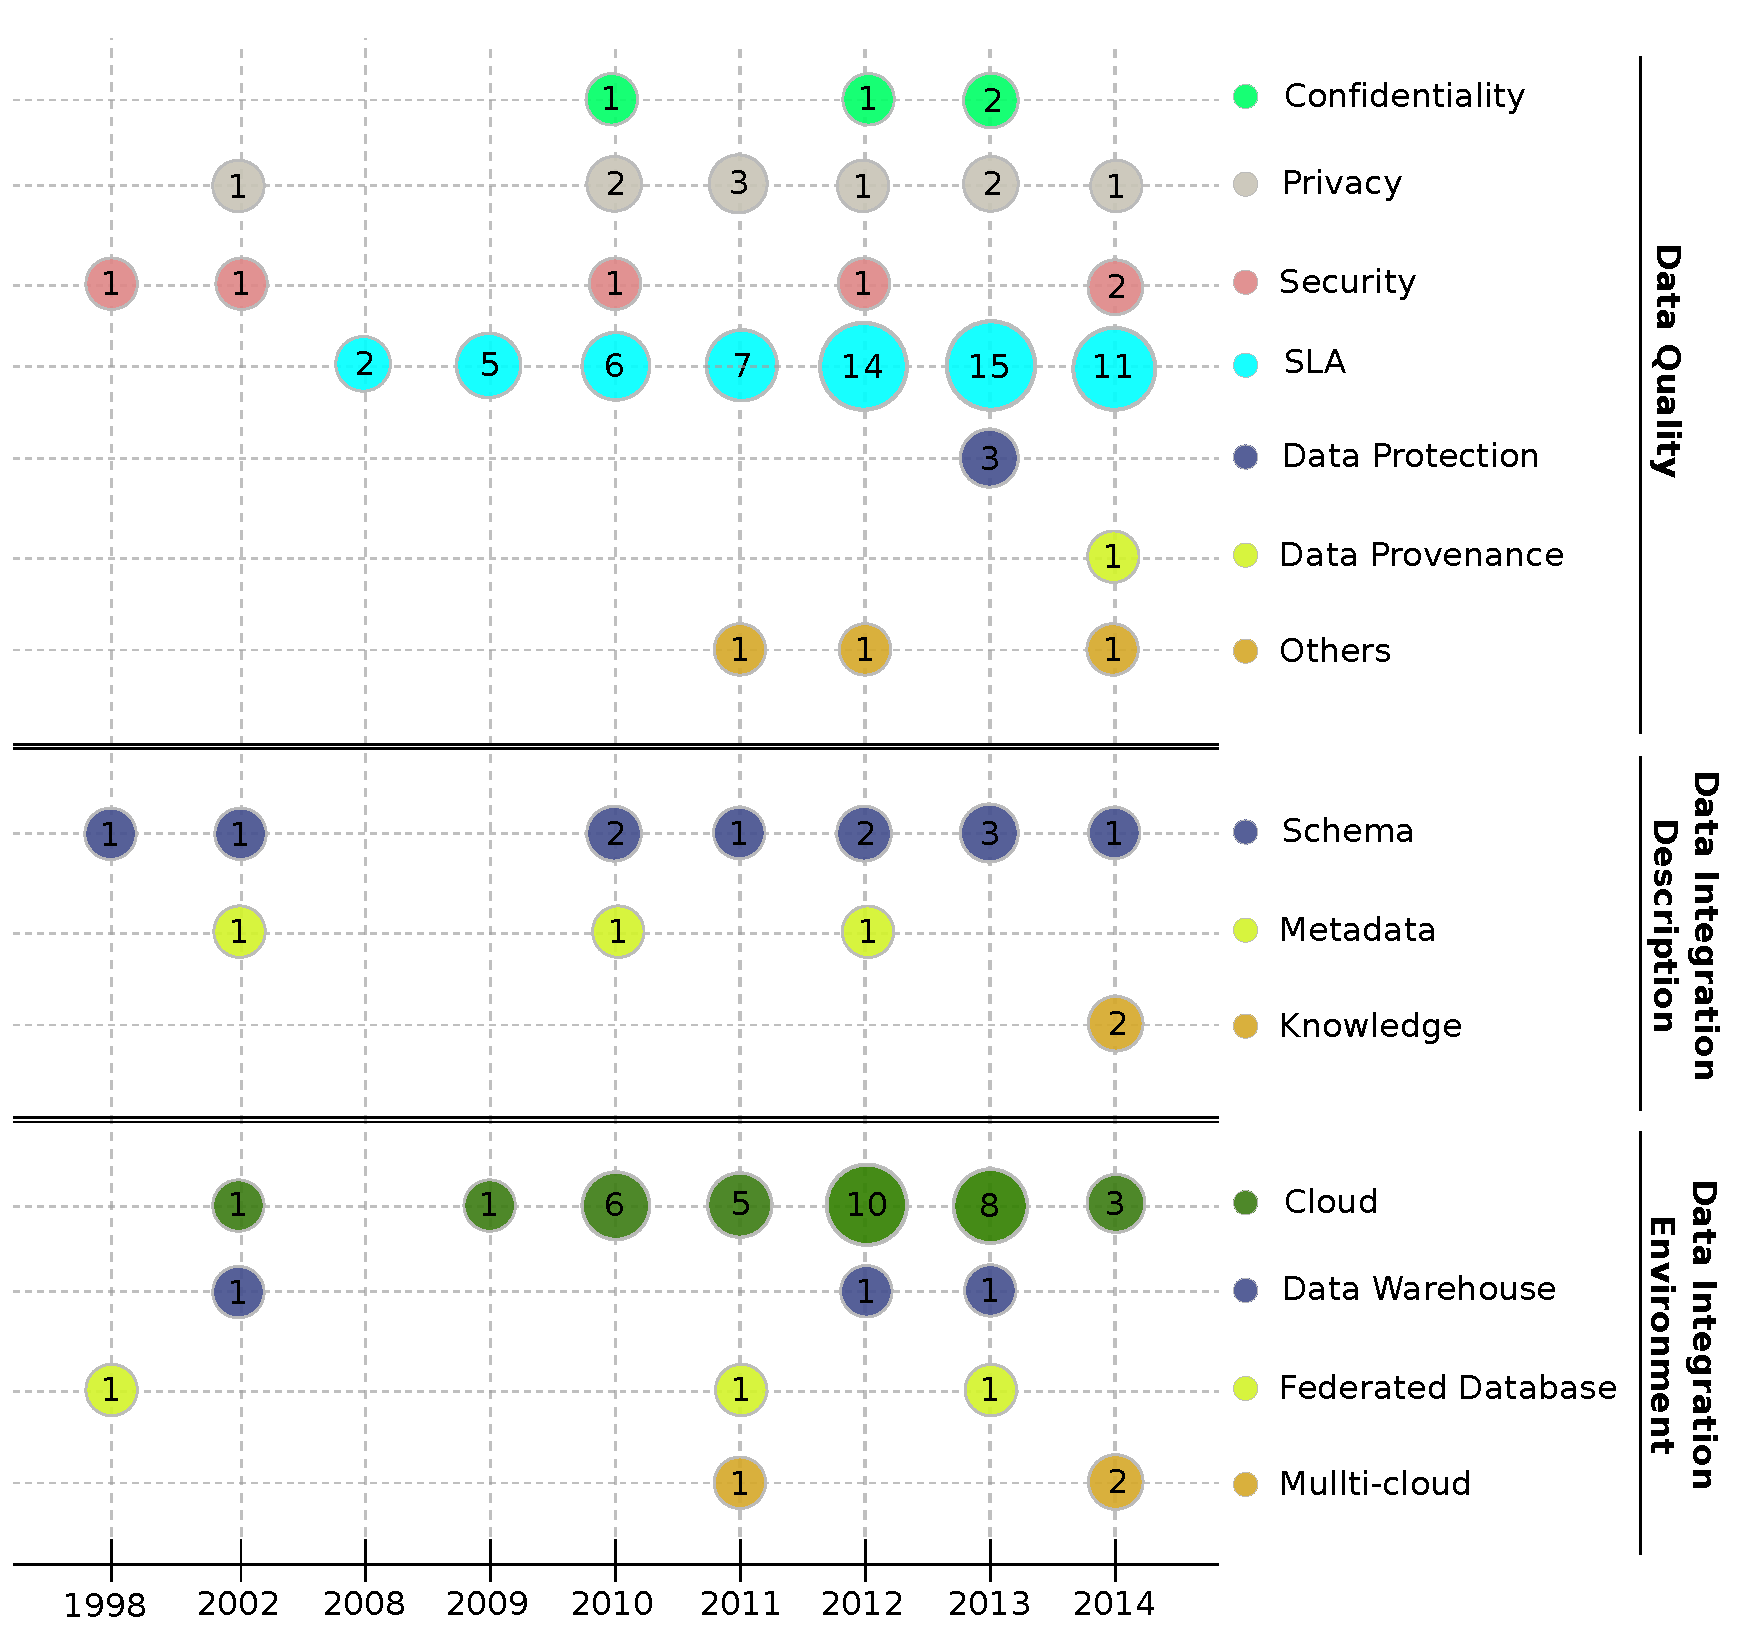
\includegraphics[scale=0.42]{figs/bubble-charts/PublicationsPerYear.pdf} 
\caption{Publications Per Year}\label{fig:pubperyear}
\end{figure}